% !TeX program = pdflatex
% =============================================================================
% Arbeitsblatt: Waagrechter Wurf (nicht bewertet, Übungsmaterial für den
% Unterricht)
% Kantonsschule KFR – Physik, 4. Klasse, 1. HS, Mechanik
%
% Kopiert aus vorlagen/arbeitsblatt-vorlage.tex und um dieselben
% Farb-/Boxdefinitionen ergänzt wie zusammengesetzte-bewegungen-arbeitsblatt.tex
% (gleicher Themencluster, direkt anschliessende Lektion). Templates sind
% selbstständig/nicht DRY, siehe CLAUDE.md.
%
% Notation: $x$ (waagrecht), $y$ (senkrecht, nach oben positiv), Ursprung auf
% dem Boden direkt unter der Abwurfstelle -- exakt dieselbe
% Vorzeichenkonvention wie in freier-fall-arbeitsblatt.tex (dort $a=-g$ bei
% "nach oben positiv"), nur jetzt mit einer zusätzlichen $x$-Koordinate.
%
% Zahlenwerte: Durchlaufendes Beispiel (h=125m, v0=10.0 m/s) sowie mehrere
% Übungsaufgaben (Wässern eines Beetes, Abwurf einer Sprengladung,
% Baderutsche, Wurfgeschwindigkeit, Aufschlag beim Volleyball,
% Verfolgungsjagd auf dem Wasser, Tennisaufschlag, Powerbiker) sind 1:1
% bzw. leicht kontextadaptiert aus den in lernziele.md referenzierten
% LEIFIphysik-Quellen übernommen und gegen deren publizierte Lösungen
% geprüft (Tennisaufschlag ist eine eigene, selbst durchgerechnete
% Verknüpfungsaufgabe, keine LEIFI-Quelle). Der Powerbiker-Aufgabenteil
% c)-e) (Bahnkurve/Auftreffgeschwindigkeit/-winkel) war in der Quelle
% hinter einem Lösungs-Klapptext verborgen und wurde deshalb selbst
% hergeleitet (v0=7.672 m/s, g*t=7.672 m/s -- beide praktisch identisch,
% daher vW=v0*sqrt(2)=10.8 m/s und der Auftreffwinkel exakt -45.0°).
%
% Einstieg: Einleitung mit Baseballpitcher-Bild (Bilder/Pitching-Mechanics.jpg)
% direkt nach den Lernzielen, gefolgt von einer Partnerarbeit mit der
% PhET-Simulation "Projektilbewegung" (Bilder/Phet_simulation.png,
% klickbarer Link statt QR-Code) -- beides noch vor der ersten
% Theoriebox. Aufschlag beim Volleyball und Verfolgungsjagd sind normale
% Übungen, keine gesonderte Vertiefungsvariante (beide lösbar mit bereits
% bekanntem Stoff, siehe lernziele.md, Implementierungsstatus). Luftwiderstand
% und Objektform/-volumen werden separat, direkt bei der
% Modellgrenzen-Theoriebox, in der Simulation untersucht.
%
% Stand: Lernziele, Theorie und Aufgaben fertig (Reihenfolge =
% Dokumentreihenfolge, stimmt mit der LZ-Nummerierung aus lernziele.md
% überein, keine Umnummerierung nötig).
% =============================================================================
\documentclass[addpoints,11pt,a4paper]{exam}

\usepackage[T1]{fontenc}
\usepackage[utf8]{inputenc}
\usepackage[ngerman]{babel}
\usepackage{lmodern}
\usepackage[a4paper,margin=2.2cm,headheight=14pt]{geometry}
\usepackage{amsmath}
\usepackage{amssymb}
\usepackage{siunitx}
% Hausstil: zusammengesetzte Einheiten immer als echter Bruch (\frac), nicht
% als Schrägstrich inline oder \tfrac. Gilt global für jedes \si/\SI.
\sisetup{per-mode=fraction,fraction-command=\frac}
\usepackage{array,booktabs,tabularx,multirow}
\usepackage{enumitem}
\usepackage{graphicx}
\usepackage{xcolor}
\usepackage{colortbl}
\usepackage{tikz}
\usepackage{physics}
\usepackage{circuitikz}
\usepackage[most]{tcolorbox}
\usepackage{lastpage}
\usepackage{needspace}
\usepackage{url}
\usepackage{hyperref}

\usetikzlibrary{arrows.meta,calc,angles,quotes}

\setlength{\parindent}{0pt}
\setlength{\parskip}{0.45em}

% -----------------------------
% Farben (Hausfarbschema Physik KFR)
% -----------------------------
\definecolor{titleblue}{HTML}{183A6B}
\definecolor{accentblue}{HTML}{2E6F9E}
\definecolor{lightblue}{HTML}{EAF4FB}
\definecolor{verylightblue}{HTML}{F7FBFE}
\definecolor{lightgray}{HTML}{F4F6F8}
\definecolor{darkgray}{HTML}{4A4A4A}
% Für Diagramme mit zwei verschiedenen Funktionen/Linien: titleblue (dunkles
% Blau) + accentorange (Orange) sind weit genug auseinander (auch in
% Graustufen/für Farbenblinde unterscheidbar), im Gegensatz zu
% titleblue+accentblue, die beide Blautöne sind.
\definecolor{accentorange}{HTML}{D9720C}
% Für Diagramme mit DREI Linien: dritte Farbe nötig, die sich sowohl von
% titleblue als auch von accentorange klar unterscheidet, auch in
% Graustufen/für Farbenblinde. Violett liegt weit genug von Blau und Orange
% entfernt, um als dritte Linie eindeutig unterscheidbar zu bleiben.
\definecolor{accentpurple}{HTML}{7B2D8E}
% Theorieblock: eigene Farbe (grün), damit er sich auf einen Blick von den
% blauen Lernziele-/Aufgaben-Boxen abhebt.
\definecolor{theorygreen}{HTML}{2E7D4F}
\definecolor{lighttheorygreen}{HTML}{EAF7EF}
% Gruppenarbeitbox: eigene Farbe (Petrol/Teal), damit Partner-/Gruppenarbeit
% sich auf einen Blick von normalen Einzelaufgaben (blau, taskbox) und vom
% Theorieblock (grün, theoriebox) abhebt.
\definecolor{groupteal}{HTML}{1B7F72}
\definecolor{lightgroupteal}{HTML}{E8F5F3}

% Klickbare Links (Simulationslink): in accentblue statt Standard-Rot/Blau,
% damit sie sich ins Hausfarbschema einfügen.
\hypersetup{colorlinks=true,urlcolor=accentblue,linkcolor=accentblue}

% -----------------------------
% Spaltentypen
% -----------------------------
\newcolumntype{Y}{>{\centering\arraybackslash}X}
\newcolumntype{P}[1]{>{\raggedright\arraybackslash}p{#1}}

% -----------------------------
% Boxen
% -----------------------------
\newtcolorbox{titlebox}{
  enhanced,
  colback=titleblue,
  colframe=titleblue,
  boxrule=0pt,
  arc=3mm,
  left=3mm,right=3mm,top=3mm,bottom=3mm
}

% exam.cls rückt die questions-Liste um die Breite von "10." (plus \labelsep)
% ein (Platz für die Nummerierung "1.", "2." ...); wir messen dieselbe Distanz
% hier unabhängig nach.
\newlength{\aufgabenindent}
\settowidth{\aufgabenindent}{10.\hskip\labelsep}

\newtcolorbox{infobox}{
  enhanced,
  breakable,
  colback=lightblue,
  colframe=accentblue,
  boxrule=0.7pt,
  arc=2mm,
  left=5mm,right=5mm,top=2mm,bottom=2mm
}

% theoriebox: wie infobox, aber grün und mit farbigem Titelbalken. Regel:
% hervorgehobene/definierte Begriffe INNERHALB einer theoriebox immer mit
% \textbf{\emph{...}} setzen (fett UND kursiv), nicht mit blossem \emph{...}.
\newtcolorbox{theoriebox}[1][Theorie]{
  enhanced,
  breakable,
  colback=lighttheorygreen,
  colframe=theorygreen,
  title={#1},
  fonttitle=\bfseries,
  boxrule=0.7pt,
  arc=2mm,
  left=5mm,right=5mm,top=2mm,bottom=2mm
}

% taskbox steht direkt in der questions-Liste (vor dem ersten \question),
% also innerhalb von deren Einrückung.
\newtcolorbox{taskbox}[1][]{
  enhanced,
  breakable,
  colback=verylightblue,
  colframe=accentblue,
  title={#1},
  fonttitle=\bfseries,
  boxrule=0.7pt,
  arc=2mm,
  enlarge left by=-\aufgabenindent,
  width=\textwidth,
  left=5mm,right=5mm,top=2mm,bottom=2mm
}

% beispielbox: wie taskbox (blau), aber ausserhalb von questions.
\newtcolorbox{beispielbox}[1][Beispiel]{
  enhanced,
  breakable,
  colback=verylightblue,
  colframe=accentblue,
  title={#1},
  fonttitle=\bfseries,
  boxrule=0.7pt,
  arc=2mm,
  left=5mm,right=5mm,top=2mm,bottom=2mm
}

% groupbox: JEDE Aufgabe mit Partner-/Gruppenarbeit bekommt diese Box statt
% der blauen taskbox. Strukturell identisch zu taskbox (gleiche
% Einrückungskorrektur, da auch groupbox innerhalb von questions steht).
\newtcolorbox{groupbox}[1][Gruppenarbeit]{
  enhanced,
  breakable,
  colback=lightgroupteal,
  colframe=groupteal,
  title={#1},
  fonttitle=\bfseries,
  boxrule=0.7pt,
  arc=2mm,
  enlarge left by=-\aufgabenindent,
  width=\textwidth,
  left=5mm,right=5mm,top=2mm,bottom=2mm
}

% hinweisbox: eigene Farbe (Orange), für wichtige Klarstellungen/Warnungen
% vor häufigen Verwechslungen.
\definecolor{lightorange}{HTML}{FCEEE0}
\newtcolorbox{hinweisbox}[1][Hinweis]{
  enhanced,
  breakable,
  colback=lightorange,
  colframe=accentorange,
  title={#1},
  fonttitle=\bfseries,
  boxrule=0.7pt,
  arc=2mm,
  left=5mm,right=5mm,top=2mm,bottom=2mm
}

% formelbox: eigene Farbe (Violett), um zentrale Formeln visuell klar von
% normaler Theorie abzuheben.
\definecolor{lightpurple}{HTML}{F3EAF7}
\newtcolorbox{formelbox}[1][Formel]{
  enhanced,
  breakable,
  colback=lightpurple,
  colframe=accentpurple,
  title={#1},
  fonttitle=\bfseries,
  boxrule=0.9pt,
  arc=2mm,
  left=5mm,right=5mm,top=2mm,bottom=2mm
}

\newtcolorbox{answerbox}{
  breakable,
  colback=white,
  colframe=gray!55,
  boxrule=0.5pt,
  arc=1.5mm,
  left=2mm,right=2mm,top=2mm,bottom=2mm
}

% --- Lösungen ein-/ausblenden -----------------------------------------------
% Schülerexemplar (Standard): \noprintanswers
% Lehrer-/Lösungsexemplar:    \printanswers
\noprintanswers
% \printanswers

% --- Punkte bleiben intern, werden aber nicht gedruckt ----------------------
\pointformat{}

% --- Lösungsbox auf Deutsch, farblich abgesetzt -----------------------------
\renewcommand{\solutiontitle}{\noindent\color{titleblue}\textbf{Lösung:}\enspace}

% --- Kopf-/Fusszeile: Thema/Titel oben, Seitenzahl unten --------------------
\pagestyle{headandfoot}
\cfoot{\textcolor{darkgray}{Seite \thepage\ von \pageref{LastPage}}}

% --- Kopfzeile: Klasse / Datum / Thema / Titel ------------------------------
\newcommand{\Kopfzeile}[4]{%
  \begin{titlebox}
    {\color{white}\sffamily\bfseries\Large #4}
  \end{titlebox}
  \vspace{0.5em}
  \noindent\textbf{Klasse:}~#1 \hfill \textbf{Datum:}~#2 \hfill \textbf{Thema:}~#3
    \hfill \textbf{Lehrperson:}~Loris Keller
  \vspace{0.8em}
  \lhead{\textcolor{darkgray}{#3}}
  \rhead{\textcolor{darkgray}{#4}}
}

% --- Antwortraum: ca. 2.5 cm Platz pro Punkt, als umrandetes Feld -----------
\newlength{\antwortraumlen}
\newcommand{\Antwortraum}[1]{%
  \pgfmathsetlength{\antwortraumlen}{#1*2.5cm}%
  \begin{answerbox}
    \rule{0pt}{\antwortraumlen}%
  \end{answerbox}%
}

% Werte für Kopfzeile zentral setzen
\newcommand{\Klasse}{4a}
\newcommand{\Datum}{02.10.2026}
\newcommand{\Thema}{Waagrechter Wurf}
\newcommand{\ArbeitsblattTitel}{Arbeitsblatt: Waagrechter Wurf}

\begin{document}

\Kopfzeile{\Klasse}{\Datum}{\Thema}{\ArbeitsblattTitel}

% --- Lernziele: aus lernziele.md (Backward-Design, Stufe 1) übernommen.
% LZ1..LZ5 entsprechen der Reihenfolge, in der die zugehörigen
% Theorieboxen/Übungen im Dokument erscheinen, keine Umnummerierung nötig.
\begin{infobox}
\textbf{Lernziele}\\
Am Ende dieser Einheit kann ich \dots
\begin{itemize}[leftmargin=1.2cm,itemsep=0.25em]
  \item erklären, dass der waagrechte Wurf die Überlagerung einer gleichförmigen Horizontalbewegung mit dem freien Fall ist (Anwendung des bekannten Unabhängigkeitsprinzips auf $v_{0y}=0$). (LZ1)
  \item für einen waagrechten Wurf aus gegebener Anfangshöhe $h$ und Anfangsgeschwindigkeit $v_0$ die Wurfzeit $t_{\text{W}}$ und die Wurfweite $w$ berechnen. (LZ2)
  \item durch Elimination der Zeit aus $x(t)$ und $y(t)$ die Gleichung der Bahnkurve $y(x)$ herleiten und für gegebene Werte aufstellen. (LZ3)
  \item die Auftreffgeschwindigkeit (Betrag, mit Pythagoras) und den Auftreffwinkel (mit Tangens) eines waagrecht geworfenen Körpers berechnen. (LZ4)
  \item benennen, welche Vereinfachungen dem Modell des waagrechten Wurfs zugrunde liegen, und qualitativ einschätzen, wie sich deren Verletzung auf das Ergebnis auswirken würde. (LZ5)
\end{itemize}
\end{infobox}

% =============================================================================
% Einleitung: Baseballpitcher als real-weltliches Beispiel eines nahezu
% waagrechten Wurfs mit hoher Geschwindigkeit, Bild aus Bilder/.
% =============================================================================
\begin{beispielbox}[Einleitung: Wie weit sinkt ein geworfener Baseball auf dem Weg zum Schlagmal?]
Ein Baseballpitcher wirft den Ball aus einer Abwurfhöhe von rund zwei
Metern nahezu waagrecht in Richtung Schlagmal, das $\SI{18.4}{\meter}$
entfernt liegt, mit Geschwindigkeiten von teilweise über
$\SI{140}{\kilo\meter\per\hour}$.

\begin{center}
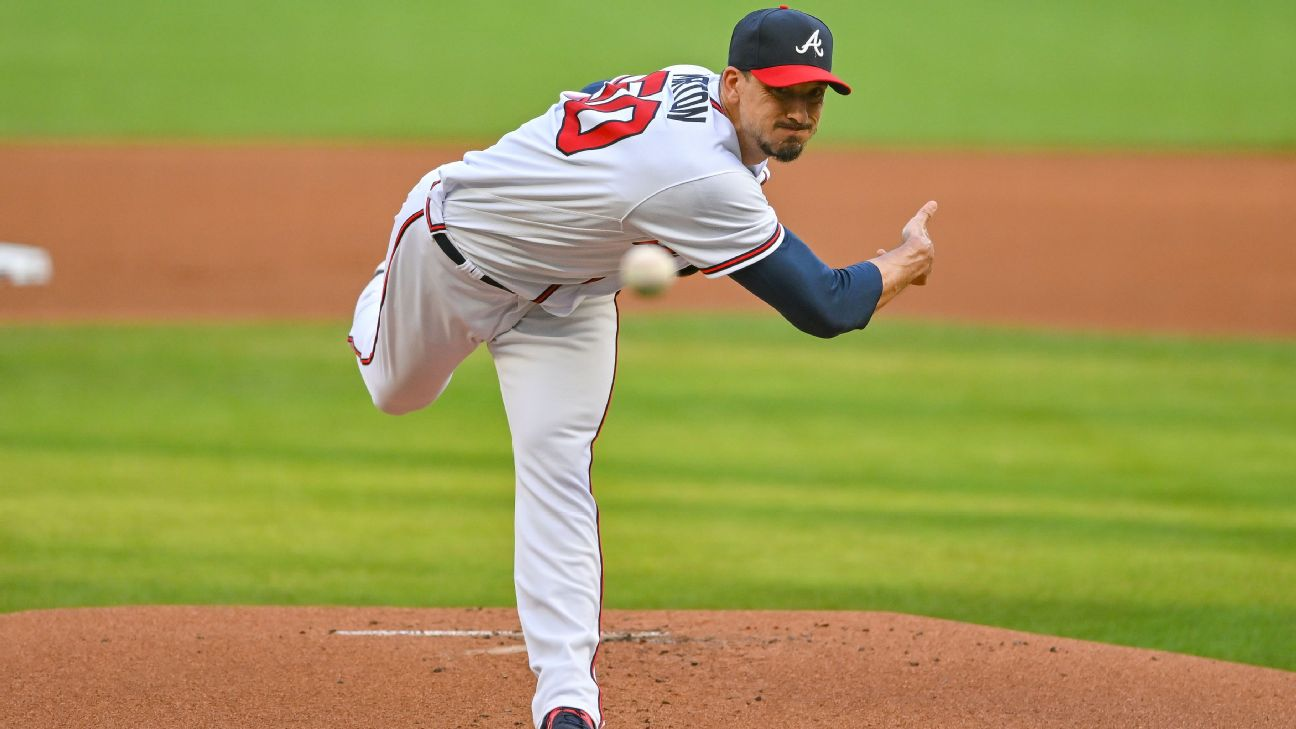
\includegraphics[width=0.55\linewidth]{Bilder/Pitching-Mechanics.jpg}
\end{center}
{\scriptsize Bewegungsablauf eines Baseballpitchers: Der Ball verlässt die
Hand nahezu waagrecht mit hoher Geschwindigkeit.}

Wie jeder waagrecht geworfene Körper folgt der Ball dabei der Schwerkraft
und sinkt während des Flugs ein Stück ab, bevor er beim Schlagmal
ankommt: Ein guter Batter kalkuliert diesen Effekt unbewusst mit ein,
sonst schlägt er zu hoch oder zu tief daneben. Auf diesem Arbeitsblatt
lernst du, wie man berechnet, wie weit ein waagrecht geworfener Körper
fliegt und wie stark er dabei absinkt, und kannst damit selbst
abschätzen, wie tief der Ball beim Pitcherwurf tatsächlich fällt.
\end{beispielbox}

\begin{groupbox}[Partnerarbeit: Simulation erkunden]
Ihr braucht zu zweit ein Gerät mit Internetzugang. Öffnet die
PhET-Simulation \glqq Projektilbewegung\grqq{} über diesen Link und
probiert die Fragen a) bis d) direkt in der Simulation aus, \textbf{bevor}
ihr weiterrechnet:

\begin{center}
\href{https://phet.colorado.edu/de/simulations/projectile-motion}{\textbf{\large phet.colorado.edu/de/simulations/projectile-motion}}
\end{center}

\begin{center}
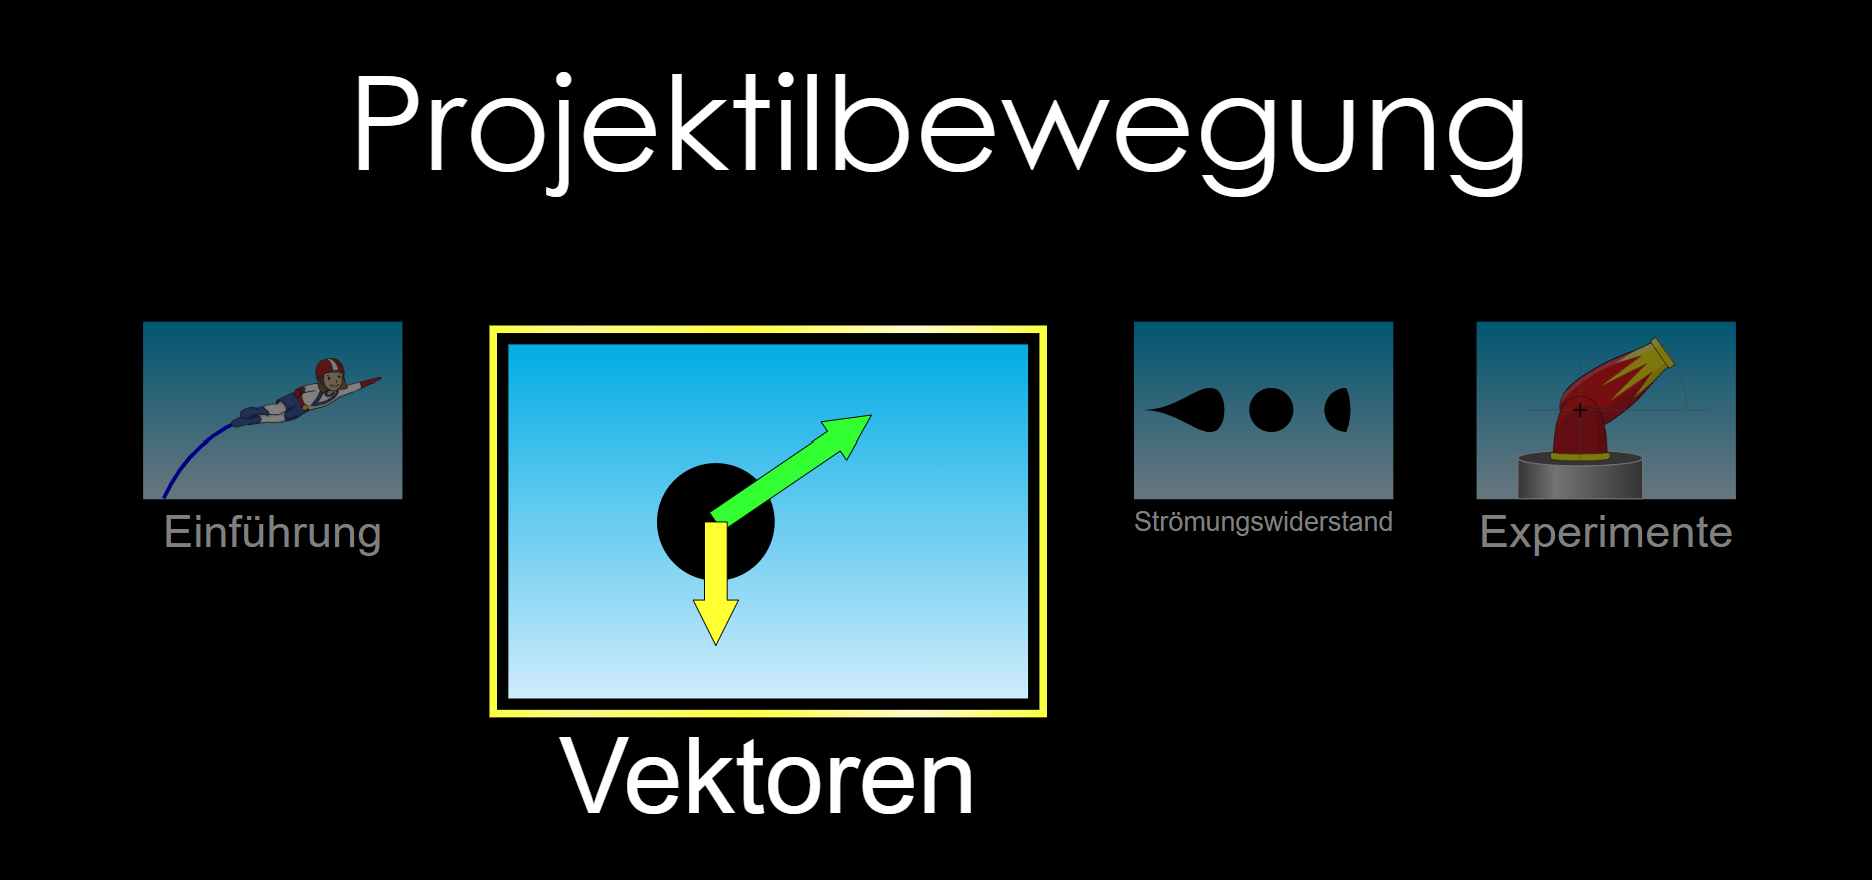
\includegraphics[width=0.6\linewidth]{Bilder/Phet_simulation.png}
\end{center}
{\scriptsize Die PhET-Simulation \glqq Projektilbewegung\grqq{}:
Abwurfwinkel, Anfangsgeschwindigkeit $v_0$, Höhe $h$, Masse und
Luftwiderstand lassen sich einzeln einstellen.}

Stellt den Abwurfwinkel auf $\SI{0}{\degree}$ (waagrecht, das Thema dieser
Einheit).

\begin{parts}
  \part[3] \textbf{Höhe:} Schaltet den Luftwiderstand aus. Testet mehrere
  Werte für die Kanonenhöhe $h$ bei jeweils gleichbleibendem $v_0$. Wie
  verändert sich die Wurfweite, wenn $h$ grösser wird?
  \Antwortraum{3}
  \begin{solution}
  Grössere $h$ $\Rightarrow$ grössere Wurfweite: Nach $t_{\text{W}} =
  \sqrt{2h/g}$ wächst die Wurfzeit mit $h$, und bei gleichbleibendem $v_0$
  wächst damit auch $w=v_0\cdot t_{\text{W}}$ (diese Formeln lernt ihr
  gleich unten formal kennen).
  \end{solution}

  \part[3] \textbf{Anfangsgeschwindigkeit:} Haltet jetzt $h$ konstant und
  testet mehrere Werte für $v_0$. Wie verändert sich die Wurfweite, wenn
  $v_0$ grösser wird?
  \Antwortraum{3}
  \begin{solution}
  Grösseres $v_0$ $\Rightarrow$ proportional grössere Wurfweite: Die
  Wurfzeit hängt nur von $h$ ab und bleibt bei konstantem $h$ gleich,
  also wächst die Wurfweite direkt proportional zu $v_0$.
  \end{solution}

  \part[2] \textbf{Masse:} Verändert bei weiterhin ausgeschaltetem
  Luftwiderstand die Masse des Geschosses (bei gleichem $h$ und $v_0$).
  Was passiert mit der Wurfweite?
  \Antwortraum{2}
  \begin{solution}
  Keine Änderung: Ohne Luftwiderstand hat die Masse keinen Einfluss auf
  die Wurfweite, genau wie schon beim freien Fall. (Was sich ändert,
  sobald der Luftwiderstand eingeschaltet ist, untersucht ihr später bei
  den Modellgrenzen.)
  \end{solution}

  \part[3] \textbf{Geschwindigkeitskomponenten:} Schaltet die Anzeige der
  Geschwindigkeitskomponenten $v_x$ und $v_y$ ein und lasst mehrere Würfe
  laufen. Wie verhält sich $v_x$ während des Flugs, wie $v_y$? Notiert
  eure Beobachtung, ihr werdet sie gleich in der Theorie unten bestätigt
  sehen.
  \Antwortraum{3}
  \begin{solution}
  $v_x$ bleibt während des ganzen Flugs konstant. $v_y$ wächst dem Betrag
  nach linear mit der Zeit, exakt wie beim freien Fall, den ihr aus der
  letzten Einheit kennt.
  \end{solution}
\end{parts}
\end{groupbox}

% =============================================================================
% Theorie: fachliche Grundlage für die Aufgaben, in eigene Boxen unterteilt,
% Reihenfolge = Lernzielreihenfolge oben. Durchlaufendes Beispiel
% (Rettungshelikopter über dem Vierwaldstättersee, h=125m, v0=10.0 m/s) aus
% der LEIFIphysik-Grundwissenseite übernommen und durch alle vier
% Theorieboxen weitergeführt.
% =============================================================================
\begin{theoriebox}[Der waagrechte Wurf: Überlagerung zweier bekannter Bewegungen]
Ein Körper wird \textbf{\emph{waagrecht}} mit der Anfangsgeschwindigkeit
$v_0$ abgeworfen (zum Beispiel ein Ball, der über eine Tischkante rollt,
oder ein Paket, das aus einem fliegenden Helikopter fällt). Nach dem
\textbf{\emph{Unabhängigkeitsprinzip}} aus der letzten Einheit überlagern
sich dabei zwei Bewegungen, die sich gegenseitig \textbf{\emph{nicht}}
beeinflussen:

\begin{itemize}[leftmargin=1.2cm,itemsep=0.2em]
  \item \textbf{\emph{Waagrecht}} ($x$-Richtung): eine \textbf{\emph{gleichförmige
  Bewegung}} mit konstanter Geschwindigkeit $v_0$, denn in dieser Richtung
  wirkt keine Beschleunigung.
  \item \textbf{\emph{Senkrecht}} ($y$-Richtung): ein ganz gewöhnlicher
  \textbf{\emph{freier Fall}} mit $a=-g$, wie du ihn aus der
  Freier-Fall-Einheit kennst, hier mit der Anfangsgeschwindigkeit $v_{0y}=0$
  (die Anfangsgeschwindigkeit zeigt ja rein waagrecht, hat also keine
  senkrechte Komponente).
\end{itemize}

Mit dem Koordinatenursprung auf dem Boden, senkrecht unter der
Abwurfstelle, und \glqq nach oben positiv\grqq{} (dieselbe Konvention wie
in der Freier-Fall-Einheit) ergibt sich, indem du die bereits bekannten
Bewegungsgleichungen einfach auf diese beiden Richtungen anwendest:
\begin{formelbox}[Bewegungsgleichungen des waagrechten Wurfs]
\[
  \boxed{x(t) = v_0 \cdot t}, \qquad \boxed{y(t) = h - \frac{1}{2}\,g\,t^2},
\]
mit der Anfangshöhe $h$ (Einheit: $\si{\meter}$) über dem Ursprung.
\end{formelbox}

\begin{hinweisbox}
Neu ist an diesen Gleichungen \textbf{nichts}: $x(t)$ ist exakt die
gleichförmige Bewegung aus den Bewegungsgleichungen, $y(t)$ ist exakt der
freie Fall aus der Ruhe (nur mit einer Anfangshöhe $h$ statt einem
Startpunkt bei null). Neu ist nur, dass \textbf{\emph{beide gleichzeitig}}
ablaufen, unabhängig voneinander.
\end{hinweisbox}

\textbf{Durchlaufendes Beispiel:} Ein Rettungshelikopter fliegt in
$h=\SI{125}{\meter}$ Höhe mit $v_0=\SI{10.0}{\meter\per\second}$ waagrecht
über den Vierwaldstättersee und lässt (im Modell ohne Luftwiderstand) ein
Hilfspaket fallen. Damit gilt für dieses Paket:
\[
  x(t) = \SI{10.0}{\meter\per\second}\cdot t, \qquad y(t) = \SI{125}{\meter} - \frac{1}{2}\cdot\SI{9.81}{\meter\per\second\squared}\cdot t^2.
\]
Dieses Beispiel begleitet dich durch die nächsten drei Theorieboxen.
\end{theoriebox}

\begin{theoriebox}[Wurfzeit und Wurfweite]
Als \textbf{\emph{Wurfzeit}} $t_{\text{W}}$ bezeichnet man die Zeit vom
Abwurf bis zum Auftreffen auf dem Boden, also bis $y(t_{\text{W}})=0$.
Das hast du im Prinzip schon in der Freier-Fall-Einheit gelöst:
\[
  0 = h - \frac{1}{2}\,g\,t_{\text{W}}^2 \quad\Longrightarrow\quad \frac{1}{2}\,g\,t_{\text{W}}^2 = h \quad\Longrightarrow\quad t_{\text{W}}^2 = \frac{2h}{g} \quad\Longrightarrow\quad \boxed{t_{\text{W}} = \sqrt{\frac{2h}{g}}}.
\]

\begin{hinweisbox}
Die Wurfzeit hängt nur von $h$ und $g$ ab, \textbf{\emph{nicht}} von $v_0$!
Ob du den Ball ganz sanft oder sehr schnell waagrecht wegwirfst: Solange
die Abwurfhöhe $h$ gleich bleibt, kommt er immer gleichzeitig unten an
(genau das Unabhängigkeitsprinzip, das du vorhin in der Simulation
beobachtet hast).
\end{hinweisbox}

Als \textbf{\emph{Wurfweite}} $w$ bezeichnet man die waagrechte Strecke,
die der Körper bis zum Auftreffen zurücklegt, also $x(t_{\text{W}})$:
\[
  \boxed{w = v_0 \cdot t_{\text{W}}}, \qquad \text{Einheit von } w\colon\ \si{\meter}.
\]

\textbf{Beispiel (Fortsetzung):} Für das Hilfspaket mit
$h=\SI{125}{\meter}$, $v_0=\SI{10.0}{\meter\per\second}$:
\[
  t_{\text{W}} = \sqrt{\frac{2\cdot\SI{125}{\meter}}{\SI{9.81}{\meter\per\second\squared}}} = \sqrt{\SI{25.5}{\second\squared}} \approx \SI{5.05}{\second}.
\]
\[
  w = \SI{10.0}{\meter\per\second}\cdot\SI{5.05}{\second} = \SI{50.5}{\meter}.
\]
\end{theoriebox}

\begin{questions}
\begin{taskbox}[Übung: Wurfzeit und Wurfweite]
\question[6] Ein Gärtner hält einen Wasserschlauch waagerecht und möchte
ein $\SI{6.0}{\meter}$ entferntes Beet wässern. Das Wasser tritt mit
$v_0=\SI{12}{\meter\per\second}$ aus dem Schlauch aus. Luftwiderstand
soll vernachlässigt werden.

\begin{parts}
  \part[3] Berechne, wie lange das Wasser vom Austritt bis zum Auftreffen
  auf das Beet braucht.
  \Antwortraum{3}
  \begin{solution}
  Hier ist die Wurfweite $w=\SI{6.0}{\meter}$ bereits gegeben (statt $h$),
  also lösen wir $w=v_0\cdot t_{\text{W}}$ nach $t_{\text{W}}$ auf:
  \[
    t_{\text{W}} = \frac{w}{v_0} = \frac{\SI{6.0}{\meter}}{\SI{12}{\meter\per\second}} = \SI{0.50}{\second}.
  \]
  \end{solution}

  \part[3] Berechne, wie hoch der Gärtner den Schlauch mindestens halten
  muss, damit das Wasser bis zum Beet gelangt.
  \Antwortraum{3}
  \begin{solution}
  Mit dem $t_{\text{W}}$ aus a) lösen wir $t_{\text{W}}=\sqrt{2h/g}$ nach
  $h$ auf:
  \[
    t_{\text{W}}^2 = \frac{2h}{g} \quad\Longrightarrow\quad h = \frac{g\cdot t_{\text{W}}^2}{2}.
  \]
  \[
    h = \frac{\SI{9.81}{\meter\per\second\squared}\cdot(\SI{0.50}{\second})^2}{2} \approx \SI{1.2}{\meter}.
  \]
  \end{solution}
\end{parts}

\question[6] Im Winter warf ein mit $v_0=\SI{720}{\kilo\meter\per\hour}$
waagrecht fliegendes Flugzeug eine Sprengladung auf einen zugefrorenen
Fluss, um dort das Eis kontrolliert aufzubrechen (eine reale Technik zur
Vermeidung von Eisstauhochwasser). Die Sprengladung hatte einen
Zeitzünder und detonierte genau $\SI{5.00}{\second}$ nach dem Abwurf beim
Aufprall auf dem Eis.

\begin{parts}
  \part[3] Berechne den horizontalen Abstand vor dem Ziel, in dem die
  Sprengladung abgeworfen werden musste.
  \Antwortraum{3}
  \begin{solution}
  \[
    v_0 = \SI{720}{\kilo\meter\per\hour} = \frac{720}{3.6}\,\si{\meter\per\second} = \SI{200}{\meter\per\second}.
  \]
  \[
    w = v_0 \cdot t_{\text{W}} = \SI{200}{\meter\per\second}\cdot\SI{5.00}{\second} = \SI{1000}{\meter}.
  \]
  \end{solution}

  \part[3] Berechne die Höhe, in der das Flugzeug beim Abwurf über dem Eis
  fliegen musste.
  \Antwortraum{3}
  \begin{solution}
  \[
    h = \frac{1}{2}\,g\,t_{\text{W}}^2 = \frac{1}{2}\cdot\SI{9.81}{\meter\per\second\squared}\cdot(\SI{5.00}{\second})^2 = \frac{1}{2}\cdot\SI{9.81}{\meter\per\second\squared}\cdot\SI{25.0}{\second\squared} \approx \SI{123}{\meter}.
  \]
  \end{solution}
\end{parts}
\end{taskbox}
\end{questions}

\begin{theoriebox}[Die Bahnkurve: Herleitung der Wurfparabel]
Die Gleichungen $x(t)$ und $y(t)$ beschreiben, \emph{wann} sich der Körper
an welchem Ort befindet. Manchmal will man aber direkt wissen: Auf welcher
\emph{Höhe} $y$ befindet sich der Körper bei einer bestimmten waagrechten
Position $x$, unabhängig von der Zeit? Dafür \textbf{\emph{eliminiert}}
man die Zeit $t$ aus den beiden Gleichungen.

\textbf{Schritt 1:} $x(t)=v_0\cdot t$ nach $t$ auflösen:
\[
  t = \frac{x}{v_0}.
\]
\textbf{Schritt 2:} Diesen Ausdruck für $t$ in $y(t)=h-\tfrac{1}{2}g t^2$
einsetzen:
\[
  y(x) = h - \frac{1}{2}\,g\,\left(\frac{x}{v_0}\right)^2.
\]
\textbf{Schritt 3:} Die Klammer ausquadrieren:
\[
  \boxed{y(x) = h - \frac{1}{2}\cdot\frac{g}{v_0^2}\cdot x^2}.
\]
Das ist die Gleichung einer nach unten geöffneten \textbf{\emph{Parabel}},
weshalb man die Bahnkurve des waagrechten Wurfs auch
\textbf{\emph{Wurfparabel}} nennt.

\begin{center}
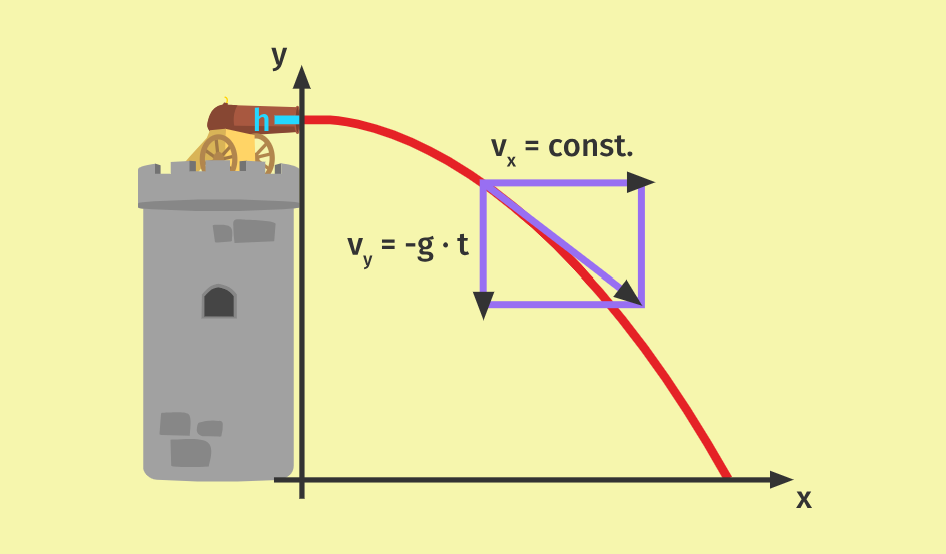
\includegraphics[width=0.62\linewidth]{Bilder/Kanone.png}
\end{center}
{\scriptsize Wurfparabel, hier für eine Kanonenkugel: $v_x$ bleibt
während des ganzen Flugs konstant, $v_y$ wächst mit der Zeit ($v_y=-gt$),
zusammen ergibt das eine Bahnkurve, die immer steiler wird.}

\begin{center}
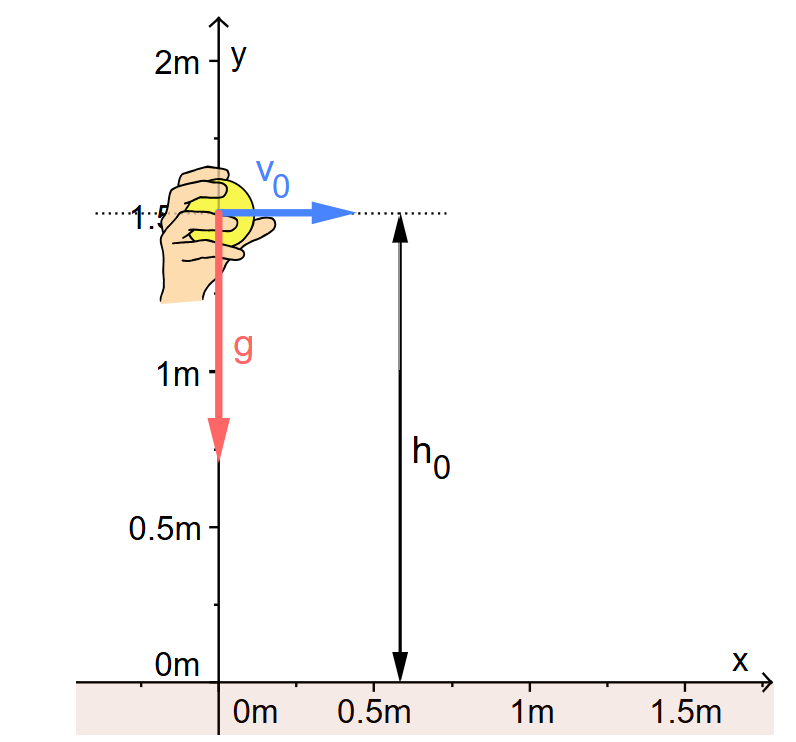
\includegraphics[width=0.5\linewidth]{Bilder/Waagrechter_Wurf.png}
\end{center}
{\scriptsize Dieselbe Idee für einen aus der Hand geworfenen Ball,
massstäblich mit Koordinatengitter: $v_0$ waagrecht, $g$ senkrecht,
Anfangshöhe $h_0$.}

\textbf{Beispiel (Fortsetzung):} Für das Hilfspaket mit
$h=\SI{125}{\meter}$, $v_0=\SI{10.0}{\meter\per\second}$:
\[
  y(x) = \SI{125}{\meter} - \frac{1}{2}\cdot\frac{\SI{9.81}{\meter\per\second\squared}}{(\SI{10.0}{\meter\per\second})^2}\cdot x^2 = \SI{125}{\meter} - \SI{0.0491}{\per\meter}\cdot x^2.
\]
\end{theoriebox}

\begin{questions}
\begin{taskbox}[Übung: Bahnkurve herleiten]
\question[4] Bestimme die Gleichung $y(x)$ der Bahnkurve für das
Wasser aus der Gärtneraufgabe von eben ($v_0=\SI{12}{\meter\per\second}$,
$h\approx\SI{1.2}{\meter}$, aus den Teilaufgaben a) und b) dort).
\Antwortraum{4}
\begin{solution}
\[
  y(x) = h - \frac{1}{2}\cdot\frac{g}{v_0^2}\cdot x^2 = \SI{1.2}{\meter} - \frac{1}{2}\cdot\frac{\SI{9.81}{\meter\per\second\squared}}{(\SI{12}{\meter\per\second})^2}\cdot x^2 \approx \SI{1.2}{\meter} - \SI{0.034}{\per\meter}\cdot x^2.
\]
\end{solution}
\end{taskbox}
\end{questions}

\begin{questions}
\begin{taskbox}[Clicker-ConcepTest: Auftreffgeschwindigkeit]
\question[3] Ein Körper wird waagrecht mit $v_0$ geworfen. Wie gross ist
seine Geschwindigkeit im Moment des Auftreffens auf dem Boden, verglichen
mit $v_0$?

\begin{parts}
  \part[3] Kreuze die richtige Aussage an und begründe sie in ein bis zwei
  Sätzen.
  \begin{itemize}[leftmargin=1.2cm,itemsep=0.15em]
    \item[$\square$] A: Genau $v_0$, denn die waagrechte Geschwindigkeit
    ändert sich ja nicht.
    \item[$\square$] B: Grösser als $v_0$, weil zusätzlich zur waagrechten
    noch eine senkrechte Geschwindigkeitskomponente dazukommt.
    \item[$\square$] C: Kleiner als $v_0$, weil die Fallbewegung die
    waagrechte Bewegung abbremst.
  \end{itemize}
  \Antwortraum{2}
  \begin{solution}
  Richtig ist \textbf{B}. Aussage A verwechselt die konstante waagrechte
  \emph{Komponente} $v_x=v_0$ mit der tatsächlichen \emph{Gesamt}geschwindigkeit:
  Beim Auftreffen ist zwar $v_x$ immer noch gleich $v_0$, aber es kommt
  eine senkrechte Komponente $v_y\neq0$ dazu (der Körper fällt ja
  gleichzeitig), und die Gesamtgeschwindigkeit ist der Betrag des
  Vektors aus beiden Komponenten, also nach Pythagoras grösser als jede
  einzelne Komponente für sich. Aussage C beruht auf der bereits
  widerlegten Vorstellung, horizontale und vertikale Bewegung würden sich
  gegenseitig beeinflussen (Unabhängigkeitsprinzip!).
  \end{solution}
\end{parts}
\end{taskbox}
\end{questions}

\begin{theoriebox}[Auftreffgeschwindigkeit und Auftreffwinkel]
Die Geschwindigkeit des Körpers zu einem beliebigen Zeitpunkt $t$ hat zwei
Komponenten:
\[
  v_x(t) = v_0 \qquad \text{(bleibt konstant)},
\]
\[
  v_y(t) = -g\cdot t \qquad \text{(wächst dem Betrag nach mit der Zeit)}.
\]
Genau wie beim rechtwinkligen Geschwindigkeitsdreieck aus der letzten
Einheit stehen diese beiden Komponenten senkrecht aufeinander, also gilt
für den \textbf{\emph{Betrag}} der Geschwindigkeit (mit Pythagoras) und
für den \textbf{\emph{Neigungswinkel}} zur Waagrechten (mit Tangens):
\begin{formelbox}[Geschwindigkeit und Winkel zu jedem Zeitpunkt]
\[
  \boxed{v(t) = \sqrt{v_0^2 + (g\,t)^2}}, \qquad \boxed{\tan(\alpha) = \frac{v_y(t)}{v_x(t)} = \frac{-g\,t}{v_0}}.
\]
\end{formelbox}
Setzt man speziell $t=t_{\text{W}}$ ein, erhält man die
\textbf{\emph{Auftreffgeschwindigkeit}} $v_{\text{W}}$ und den
\textbf{\emph{Auftreffwinkel}} $\alpha_{\text{W}}$ (das negative Vorzeichen
bedeutet dabei: der Winkel liegt \emph{unterhalb} der Waagrechten, der
Körper sinkt):
\[
  \boxed{v_{\text{W}} = \sqrt{v_0^2 + (g\,t_{\text{W}})^2}}, \qquad \boxed{\tan(\alpha_{\text{W}}) = \frac{-g\,t_{\text{W}}}{v_0}}.
\]

\begin{hinweisbox}
Achte auf den Unterschied: $v_0$ ist die \textbf{\emph{Abwurfgeschwindigkeit}}
(nur waagrecht), $v_{\text{W}}$ die \textbf{\emph{Auftreffgeschwindigkeit}}
(waagrecht \emph{und} senkrecht zusammen). Wie im Clicker-Test gerade
gezeigt, sind das \textbf{\emph{nicht}} dieselbe Grösse.
\end{hinweisbox}

\textbf{Beispiel (Fortsetzung):} Für das Hilfspaket mit
$v_0=\SI{10.0}{\meter\per\second}$ und $t_{\text{W}}=\SI{5.05}{\second}$:
\[
  v_{\text{W}} = \sqrt{(\SI{10.0}{\meter\per\second})^2 + (\SI{9.81}{\meter\per\second\squared}\cdot\SI{5.05}{\second})^2}
\]
\[
  v_{\text{W}} = \sqrt{\SI{100}{\meter\squared\per\second\squared} + \SI{2454}{\meter\squared\per\second\squared}} = \sqrt{\SI{2554}{\meter\squared\per\second\squared}} \approx \SI{50.5}{\meter\per\second}.
\]
\[
  \tan(\alpha_{\text{W}}) = \frac{-\SI{9.81}{\meter\per\second\squared}\cdot\SI{5.05}{\second}}{\SI{10.0}{\meter\per\second}} = \frac{-\SI{49.5}{\meter\per\second}}{\SI{10.0}{\meter\per\second}} = -4.95
\]
\[
  \alpha_{\text{W}} = \arctan(-4.95) \approx \SI{-78.6}{\degree}.
\]
Das Paket schlägt also mit rund $\SI{50.5}{\meter\per\second}$
($\approx\SI{182}{\kilo\meter\per\hour}$) in einem sehr steilen Winkel von
$\SI{78.6}{\degree}$ unter der Waagrechten auf, fast senkrecht: Kein
Zufall, denn nach $\SI{5.05}{\second}$ Fallzeit ist $v_y$ mit fast
$\SI{49.5}{\meter\per\second}$ schon viel grösser als das konstante
$v_0=\SI{10}{\meter\per\second}$.
\end{theoriebox}

\begin{questions}
\begin{taskbox}[Übung: Auftreffgeschwindigkeit und -winkel]
\question[6] \textbf{Umgekehrt gerechnet:} Ein Kind rutscht in einem
Schwimmbad eine Rutsche hinunter und verlässt sie waagrecht,
$\SI{1.5}{\meter}$ über dem Wasser. Es trifft $\SI{2.0}{\meter}$ weiter
auf das Wasser.

\begin{parts}
  \part[3] Berechne zuerst die Zeit, die das Kind für den Flug braucht.
  \Antwortraum{3}
  \begin{solution}
  \[
    t_{\text{W}} = \sqrt{\frac{2\cdot\SI{1.5}{\meter}}{\SI{9.81}{\meter\per\second\squared}}} \approx \sqrt{\SI{0.306}{\second\squared}} \approx \SI{0.55}{\second}.
  \]
  \end{solution}

  \part[3] Berechne daraus die Geschwindigkeit, mit der das Kind die
  Rutsche verlässt (löse $w=v_0\cdot t_{\text{W}}$ nach $v_0$ auf).
  \Antwortraum{3}
  \begin{solution}
  \[
    v_0 = \frac{w}{t_{\text{W}}} = \frac{\SI{2.0}{\meter}}{\SI{0.55}{\second}} \approx \SI{3.6}{\meter\per\second} \approx \SI{13}{\kilo\meter\per\hour}.
  \]
  \end{solution}
\end{parts}

\question[3] \textbf{Multiple Choice:} Ein Junge wirft einen Stein
waagrecht von einem $\SI{5}{\meter}$ hohen Hügel weg. Der Stein fliegt
über eine waagrechte Strecke von $\SI{20}{\meter}$. Wie schnell warf der
Junge den Stein?

\begin{parts}
  \part[3] Kreuze die richtige Antwort an und begründe sie kurz (Tipp:
  Überlege zuerst, wie lange der Fall aus $\SI{5}{\meter}$ dauert, ohne
  zu rechnen).
  \begin{itemize}[leftmargin=1.2cm,itemsep=0.1em]
    \item[$\square$] a) $\SI{10}{\meter\per\second}$ \hfill
    $\square$ b) $\SI{20}{\meter\per\second}$ \hfill
    $\square$ c) $\SI{25}{\meter\per\second}$
    \item[$\square$] d) $\SI{30}{\meter\per\second}$ \hfill
    $\square$ e) Mit diesen Angaben nicht lösbar.
  \end{itemize}
  \Antwortraum{3}
  \begin{solution}
  Richtig ist \textbf{b)}. Da der Stein rein waagrecht geworfen wurde
  ($v_{0y}=0$), ist seine Fallzeit exakt dieselbe wie bei einem einfach
  fallengelassenen Stein aus $\SI{5}{\meter}$ Höhe, unabhängig von $v_0$
  (Unabhängigkeitsprinzip). Diese Zeit lässt sich für $\SI{5}{\meter}$ im
  Kopf abschätzen: $t_{\text{W}}=\sqrt{\frac{2\cdot\SI{5}{\meter}}{\SI{9.81}{\meter\per\second\squared}}}\approx\SI{1.0}{\second}$.
  Mit $w=\SI{20}{\meter}$ in $\SI{1.0}{\second}$ ergibt sich
  $v_0=w/t_{\text{W}}\approx\SI{20}{\meter\per\second}$.
  \end{solution}
\end{parts}
\end{taskbox}
\end{questions}

% =============================================================================
% Partnerpuzzle: waagrechter Wurf (v0y=0) vs. freier Fall (v0x=0) als zwei
% Spezialfälle derselben allgemeinen Bewegungsgleichungen, direkt aus
% lernziele.md übernommen. Schliesst den Bogen zurück zur
% bewegungsgleichungen-Einheit.
% =============================================================================
\begin{questions}
\begin{groupbox}[Partnerpuzzle: Waagrechter Wurf und freier Fall im Vergleich]
Beide, der waagrechte Wurf und der freie Fall, sind eigentlich nur
\textbf{\emph{Spezialfälle}} derselben allgemeinen Bewegungsgleichungen
$x(t)=x_0+v_{0x}(t-t_0)$, $y(t)=y_0+v_{0y}(t-t_0)-\tfrac{1}{2}g(t-t_0)^2$
aus der Einheit zu den Bewegungsgleichungen, nur mit unterschiedlicher
Richtung der Anfangsgeschwindigkeit.

\begin{parts}
  \part[3] Bildet Zweiergruppen. Person A erklärt Person B in eigenen
  Worten: Was ist beim waagrechten Wurf $v_{0x}$, was ist $v_{0y}$, und
  warum verschwindet dadurch ein Term in $y(t)$?
  \Antwortraum{3}

  \part[3] Person B erklärt Person A: Was ist beim freien Fall $v_{0x}$,
  was ist $v_{0y}$, und warum verschwindet dadurch ein Term in $x(t)$?
  \Antwortraum{3}

  \part[2] Gemeinsam: Gibt es eine Bewegung, die \textbf{\emph{beide}}
  Spezialfälle gleichzeitig ist ($v_{0x}=0$ und $v_{0y}=0$)? Was für eine
  Bewegung wäre das?
  \Antwortraum{2}
  \begin{solution}
  a) Beim waagrechten Wurf ist $v_{0x}=v_0$ (die Abwurfgeschwindigkeit,
  ungleich null) und $v_{0y}=0$ (kein senkrechter Anteil beim Abwurf).
  Weil $v_{0y}=0$ ist, fällt der Term $v_{0y}(t-t_0)$ in der allgemeinen
  Gleichung für $y(t)$ weg, es bleibt nur $y(t)=y_0-\tfrac{1}{2}g(t-t_0)^2$
  übrig, exakt die Formel aus der Theoriebox oben.

  b) Beim freien Fall ist $v_{0x}=0$ (keine waagrechte Bewegung) und
  $v_{0y}$ entweder $0$ (freier Fall aus der Ruhe) oder ungleich null
  (Wurf nach oben, aus der letzten Einheit bekannt). Weil $v_{0x}=0$ ist,
  fällt der Term $v_{0x}(t-t_0)$ in der allgemeinen Gleichung für $x(t)$
  weg, es bleibt $x(t)=x_0$ übrig: Die $x$-Koordinate ändert sich gar
  nicht, die Bewegung findet nur senkrecht statt.

  c) Ja: Wenn $v_{0x}=0$ \emph{und} $v_{0y}=0$ gilt, bewegt sich der
  Körper weder waagrecht noch hat er eine senkrechte Anfangsgeschwindigkeit,
  er startet also einfach in Ruhe und fällt senkrecht nach unten: der
  freie Fall aus der Ruhe, der Spezialfall des Spezialfalls.
  \end{solution}
\end{parts}
\end{groupbox}
\end{questions}

\begin{theoriebox}[Modellgrenzen: Was dieses Modell nicht mitrechnet]
Alle Formeln auf diesem Arbeitsblatt beruhen auf zwei
\textbf{\emph{Vereinfachungen}}:

\begin{itemize}[leftmargin=1.2cm,itemsep=0.2em]
  \item \textbf{\emph{Kein Luftwiderstand:}} In Wirklichkeit bremst die
  Luft einen fliegenden Körper ab, besonders bei hohen Geschwindigkeiten
  und bei leichten, grossflächigen Objekten (ein Basketball wird stärker
  gebremst als eine Bleikugel gleicher Grösse). Dadurch wird die
  tatsächliche Wurfweite \textbf{\emph{kleiner}} als die hier berechnete.
  \item \textbf{\emph{Massenpunkt:}} Wir behandeln den geworfenen Körper
  als Punkt ohne eigene Ausdehnung. Bei einem Ball mit spürbarem Radius
  müsste man eigentlich unterscheiden, ob sich $h$ auf den Mittelpunkt
  oder auf die Unterkante des Balls bezieht, das macht bei einem
  kleinen Stein kaum einen Unterschied, bei einem grossen Ball schon.
\end{itemize}

\begin{hinweisbox}
Ein idealisiertes Ergebnis ist deshalb \textbf{nicht} automatisch
\glqq falsch\grqq{} oder unrealistisch: Es beschreibt exakt, was im
Modell ohne diese Effekte passieren würde, und ist meistens eine gute
Näherung für kompakte, schwere Körper bei nicht zu hohen Geschwindigkeiten
(zum Beispiel einen Stein). Bei einem sehr leichten Objekt (Federball,
Tischtennisball) oder bei sehr hohen Geschwindigkeiten weicht die Realität
dagegen spürbar vom Modell ab.
\end{hinweisbox}
\end{theoriebox}

\begin{questions}
\begin{groupbox}[Partnerarbeit: Luftwiderstand und Form in der Simulation]
Öffnet erneut die PhET-Simulation \glqq Projektilbewegung\grqq{}:
\begin{center}
\href{https://phet.colorado.edu/de/simulations/projectile-motion}{\textbf{\large phet.colorado.edu/de/simulations/projectile-motion}}
\end{center}
Schaltet diesmal den Luftwiderstand \textbf{ein} und verändert bei
gleichem $v_0$ und $h$ sowohl die Masse als auch das Volumen (die
Grösse bzw. den Durchmesser) des Geschosses.

\begin{parts}
  \part[4] Was beobachtet ihr bei der Wurfweite, wenn ihr Masse und
  Volumen unabhängig voneinander verändert? Vergleicht insbesondere ein
  kleines, schweres Geschoss mit einem grossen, leichten Geschoss.
  \Antwortraum{4}
  \begin{solution}
  Mit eingeschaltetem Luftwiderstand fliegt ein kleines, schweres
  Geschoss deutlich weiter als ein grosses, leichtes: Der Luftwiderstand
  hängt von der Querschnittsfläche (also vom Volumen bzw. Durchmesser)
  ab, nicht direkt von der Masse. Eine grosse Fläche bei kleiner Masse
  bedeutet eine starke Abbremsung im Verhältnis zur Trägheit des Körpers,
  eine kleine Fläche bei grosser Masse dagegen kaum spürbare Abbremsung.
  \end{solution}

  \part[2] Wie passt eure Beobachtung zur Theoriebox \glqq
  Modellgrenzen\grqq{} oben? Nennt ein Beispiel aus dem Alltag, bei dem
  dieser Unterschied deutlich sichtbar wird.
  \Antwortraum{2}
  \begin{solution}
  Genau das steht in der Theoriebox oben: Ein leichtes, grossflächiges
  Objekt (zum Beispiel ein Federball oder ein Tischtennisball) weicht
  stärker vom idealisierten Modell ohne Luftwiderstand ab als ein
  kompakter, schwerer Körper (zum Beispiel ein Stein oder eine
  Bleikugel), weil bei ähnlichem Volumen mehr Masse eine relativ kleinere
  Bremswirkung durch den Luftwiderstand bedeutet.
  \end{solution}
\end{parts}
\end{groupbox}
\end{questions}

% =============================================================================
% Zwei Übungen, die mehrere der obigen Formeln hintereinander und teils
% rückwärts anwenden: Aufschlag beim Volleyball und Verfolgungsjagd auf
% dem Wasser, beide 1:1 bzw. leicht angepasst aus in lernziele.md
% referenzierten Quellen.
% =============================================================================
\begin{questions}
\begin{taskbox}[Übung: Aufschlag beim Volleyball]
\question[10] Sehr gute Volleyballspielerinnen können den Ball beim
Aufschlag auf $v_0=\SI{140}{\kilo\meter\per\hour}$ beschleunigen. Das Netz
steht $x_{\text{N}}=\SI{9.00}{\meter}$ vor der Aufschlaglinie und ist
$y_{\text{N}}=\SI{2.43}{\meter}$ hoch. Für die Teilaufgaben a) und b)
vernachlässigen wir die Grösse und den Luftwiderstand des Balls.

\begin{parts}
  \part[4] Berechne, aus welcher Höhe $h$ der Ball abgeschlagen werden
  muss, damit er das Netz gerade so überquert (Hinweis: Berechne zuerst
  die Zeit $t_{\text{N}}$ bis zum Netz aus $x_{\text{N}}$ und $v_0$, und
  löse dann $y(t_{\text{N}})=y_{\text{N}}$ nach $h$ auf).
  \Antwortraum{4}
  \begin{solution}
  \[
    v_0 = \SI{140}{\kilo\meter\per\hour} \approx \SI{38.9}{\meter\per\second}, \qquad t_{\text{N}} = \frac{x_{\text{N}}}{v_0} = \frac{\SI{9.00}{\meter}}{\SI{38.9}{\meter\per\second}} \approx \SI{0.231}{\second}.
  \]
  \[
    y_{\text{N}} = h - \frac{1}{2}\,g\,t_{\text{N}}^2 \quad\Longrightarrow\quad h = y_{\text{N}} + \frac{1}{2}\,g\,t_{\text{N}}^2
  \]
  \[
    h = \SI{2.43}{\meter} + \frac{1}{2}\cdot\SI{9.81}{\meter\per\second\squared}\cdot(\SI{0.231}{\second})^2 \approx \SI{2.69}{\meter}.
  \]
  \end{solution}

  \part[4] Ein Volleyballfeld ist auf jeder Seite $\SI{9.00}{\meter}$ tief.
  Prüfe, ob ein Ball, der mit diesem $v_0$ und dieser Abwurfhöhe $h$
  aufgeschlagen wird, im gegnerischen Feld auftrifft (also zwischen
  $x=\SI{9.00}{\meter}$ und $x=\SI{18.0}{\meter}$).
  \Antwortraum{4}
  \begin{solution}
  \[
    t_{\text{W}} = \sqrt{\frac{2\cdot\SI{2.69}{\meter}}{\SI{9.81}{\meter\per\second\squared}}} \approx \SI{0.741}{\second}, \qquad w = v_0\cdot t_{\text{W}} = \SI{38.9}{\meter\per\second}\cdot\SI{0.741}{\second} \approx \SI{28.8}{\meter}.
  \]
  Der Ball trifft bei $x\approx\SI{28.8}{\meter}$ auf, also mehr als
  $\SI{10}{\meter}$ \emph{hinter} dem gegnerischen Feld ($x=\SI{18.0}{\meter}$):
  Ganz flach und mit voller Kraft aufgeschlagen, würde der Ball weit
  ausserhalb des Feldes landen.
  \end{solution}

  \part[2] Erkläre in ein bis zwei Sätzen, wie sehr gute Spielerinnen es
  trotzdem schaffen, den Ball mit so hohem $v_0$ ins gegnerische Feld zu
  platzieren, obwohl unsere Rechnung oben etwas anderes ergibt.
  \Antwortraum{2}
  \begin{solution}
  In der Rechnung wurde ein rein \emph{waagrechter} Aufschlag angenommen.
  Tatsächlich schlagen gute Spielerinnen den Ball entweder aus grösserer
  Höhe leicht \emph{nach unten geneigt} auf (oft zusätzlich mit Topspin),
  oder sie springen ab und schlagen näher am Netz auf: Beides verkürzt
  die Flugzeit bis zum Boden und damit die Wurfweite, sodass der Ball
  trotz hohem $v_0$ im Feld bleibt. Unser Modell (rein waagrecht, kein
  Luftwiderstand) ist hier eine bewusste Vereinfachung, keine exakte
  Beschreibung eines echten Aufschlags.
  \end{solution}
\end{parts}
\end{taskbox}
\end{questions}

\begin{questions}
\begin{taskbox}[Übung: Verfolgungsjagd auf dem Wasser]
\question[10] Ein Stuntfahrer rast mit seinem Motorrad über einen
Landungssteg, der $\SI{4}{\meter}$ über der Wasseroberfläche verläuft. Er
will auf ein $\SI{5}{\meter}$ langes Boot springen, dessen Landefläche
$\SI{0.5}{\meter}$ über dem Wasser liegt. Im Moment des Absprungs ist das
Boot $e=\SI{10}{\meter}$ vom Steg entfernt und bewegt sich mit konstant
$v_{\text{B}}=\SI{30}{\kilo\meter\per\hour}\approx\SI{8.33}{\meter\per\second}$
vom Steg weg. Luftwiderstand wird vernachlässigt.

\begin{hinweisbox}
Wie schon in \glqq Zusammengesetzte Bewegungen\grqq{}: Das Boot bewegt
sich \textbf{\emph{während des Sprungs weiter}}. Rechne deshalb zuerst
wie gewohnt mit dem ruhenden Steg als Bezugssystem, und berücksichtige die
Bewegung des Bootes erst am Schluss, indem du seine zusätzlich
zurückgelegte Strecke zur ursprünglichen Distanz $e$ addierst.
\end{hinweisbox}

\begin{parts}
  \part[3] Berechne zuerst die Falltiefe $\Delta y$ vom Absprungpunkt bis
  zur Landefläche des Bootes, und daraus die Flugzeit $t_0$.
  \Antwortraum{3}
  \begin{solution}
  \[
    \Delta y = \SI{4}{\meter} - \SI{0.5}{\meter} = \SI{3.5}{\meter}, \qquad t_0 = \sqrt{\frac{2\cdot\SI{3.5}{\meter}}{\SI{9.81}{\meter\per\second\squared}}} \approx \SI{0.845}{\second}.
  \]
  \end{solution}

  \part[4] Berechne die \emph{minimale} Absprunggeschwindigkeit, bei der
  der Stuntfahrer gerade noch das \emph{hintere} Ende des Bootes erreicht
  (Hinweis: Bis zum Aufprall hat sich das Boot zusätzlich um
  $v_{\text{B}}\cdot t_0$ weiterbewegt, addiere das zu $e$).
  \Antwortraum{4}
  \begin{solution}
  Nötiger horizontaler Flugweg: $s_{\min} = e + v_{\text{B}}\cdot t_0$.
  Daraus die Geschwindigkeit $v_{\min}=s_{\min}/t_0 = e/t_0 + v_{\text{B}}$:
  \[
    v_{\min} = \frac{\SI{10}{\meter}}{\SI{0.845}{\second}} + \SI{8.33}{\meter\per\second} \approx \SI{11.8}{\meter\per\second} + \SI{8.33}{\meter\per\second} \approx \SI{20.2}{\meter\per\second} \approx \SI{73}{\kilo\meter\per\hour}.
  \]
  \end{solution}

  \part[3] Berechne analog die \emph{maximale} Absprunggeschwindigkeit,
  bei der er gerade noch auf der \emph{vorderen} Spitze des Bootes landet
  (also die Bootslänge zusätzlich berücksichtigt).
  \Antwortraum{3}
  \begin{solution}
  \[
    v_{\max} = \frac{e+l}{t_0} + v_{\text{B}} = \frac{\SI{10}{\meter}+\SI{5}{\meter}}{\SI{0.845}{\second}} + \SI{8.33}{\meter\per\second} \approx \SI{17.8}{\meter\per\second} + \SI{8.33}{\meter\per\second} \approx \SI{26.1}{\meter\per\second} \approx \SI{94}{\kilo\meter\per\hour}.
  \]
  Der Stuntfahrer muss also mit einer Geschwindigkeit zwischen etwa
  $\SI{73}{\kilo\meter\per\hour}$ und $\SI{94}{\kilo\meter\per\hour}$
  abspringen, um sicher auf dem Boot zu landen.
  \end{solution}
\end{parts}
\end{taskbox}
\end{questions}

% =============================================================================
% Tennisaufschlag: verknüpft den senkrechten Wurf nach oben aus der
% Freier-Fall-Einheit (Toss) mit dem waagrechten Wurf dieser Einheit
% (Schlag im höchsten Punkt der Flugbahn), als abschliessende Synthese
% vor der Hausaufgabe.
% =============================================================================
\begin{questions}
\begin{taskbox}[Übung: Tennisaufschlag]
\question[12] Beim Tennisaufschlag wirft die Spielerin den Ball zunächst
aus einer Höhe von $h_0=\SI{1.50}{\meter}$ mit
$v_0=\SI{4.00}{\meter\per\second}$ senkrecht nach oben (\glqq Toss\grqq{}),
genau wie beim senkrechten Wurf aus der Freier-Fall-Einheit. Am höchsten
Punkt der Flugbahn trifft der Schläger den Ball und beschleunigt ihn auf
$v_{\text{H}}=\SI{25.0}{\meter\per\second}$ waagrecht in Richtung Netz.
Luftwiderstand wird vernachlässigt.

\begin{parts}
  \part[3] Berechne die Steigzeit $t_S$ des Hochwurfs und die dabei
  zusätzlich gewonnene Höhe $\Delta h$ (mit den Formeln für den
  senkrechten Wurf nach oben aus der Freier-Fall-Einheit).
  \Antwortraum{3}
  \begin{solution}
  \[
    t_S = \frac{v_0}{g} = \frac{\SI{4.00}{\meter\per\second}}{\SI{9.81}{\meter\per\second\squared}} \approx \SI{0.408}{\second}.
  \]
  \[
    \Delta h = v_0\cdot t_S - \frac{1}{2}\,g\,t_S^2 = \SI{4.00}{\meter\per\second}\cdot\SI{0.408}{\second} - \frac{1}{2}\cdot\SI{9.81}{\meter\per\second\squared}\cdot(\SI{0.408}{\second})^2
  \]
  \[
    \Delta h \approx \SI{1.632}{\meter} - \SI{0.816}{\meter} \approx \SI{0.816}{\meter}.
  \]
  \end{solution}

  \part[2] Bestimme die Höhe $h$, auf der der Schläger den Ball trifft
  (Abwurfhöhe $h_0$ plus die in a) berechnete Zusatzhöhe $\Delta h$).
  \Antwortraum{2}
  \begin{solution}
  \[
    h = h_0 + \Delta h = \SI{1.50}{\meter} + \SI{0.816}{\meter} \approx \SI{2.32}{\meter}.
  \]
  \end{solution}

  \part[2] Begründe in ein bis zwei Sätzen, warum der Ball ab dem
  Treffmoment wie bei einem \emph{waagrechten} Wurf behandelt werden
  darf, obwohl er kurz zuvor noch eine rein senkrechte Bewegung
  ausgeführt hat.
  \Antwortraum{2}
  \begin{solution}
  Am höchsten Punkt einer Wurfbewegung ist die Geschwindigkeit für einen
  Moment $v=0$ (der Umkehrpunkt aus der Freier-Fall-Einheit): Der Ball
  hat in diesem Moment also keine vertikale Geschwindigkeit mehr, nur
  noch die vom Schläger neu aufgeprägte horizontale Geschwindigkeit
  $v_{\text{H}}$. Genau das ist die Ausgangslage des waagrechten Wurfs:
  eine rein waagrechte Anfangsgeschwindigkeit ($v_{0y}=0$) aus einer
  bestimmten Höhe.
  \end{solution}

  \part[3] Berechne mit $v_0=v_{\text{H}}$ und der Treffhöhe $h$ aus b)
  die Wurfzeit $t_{\text{W}}$ bis der Ball den Boden erreicht, und daraus
  die Wurfweite $w$.
  \Antwortraum{3}
  \begin{solution}
  \[
    t_{\text{W}} = \sqrt{\frac{2h}{g}} = \sqrt{\frac{2\cdot\SI{2.32}{\meter}}{\SI{9.81}{\meter\per\second\squared}}} \approx \SI{0.687}{\second}.
  \]
  \[
    w = v_{\text{H}}\cdot t_{\text{W}} = \SI{25.0}{\meter\per\second}\cdot\SI{0.687}{\second} \approx \SI{17.2}{\meter}.
  \]
  \end{solution}

  \part[2] Ein Tennisfeld ist von der Grundlinie bis zum Netz
  $\SI{11.9}{\meter}$ lang. Vergleiche deine berechnete Wurfweite mit
  dieser Distanz: Warum landet ein echter Aufschlag trotzdem meistens im
  gegnerischen Feld und nicht weit dahinter, obwohl unser Modell eine so
  grosse Wurfweite liefert?
  \Antwortraum{2}
  \begin{solution}
  Unser Modell nimmt einen rein waagrechten Treffer an, bei dem der Ball
  erst nach $\SI{17.2}{\meter}$ auf den Boden träfe, deutlich weiter als
  die $\SI{11.9}{\meter}$ bis zum Netz. Ein echter Aufschlag wird deshalb
  leicht \emph{nach unten geneigt} geschlagen statt rein waagrecht wie in
  unserem Modell: Das verkürzt die tatsächliche Flugstrecke, sodass der
  Ball schon im gegnerischen Aufschlagfeld auftrifft, statt weit
  dahinter.
  \end{solution}
\end{parts}
\end{taskbox}
\end{questions}

% =============================================================================
% Hausaufgabe: Powerbiker, vollständig aus lernziele.md referenzierter
% Quelle übernommen. Teile c)-e) waren dort hinter einem Lösungs-Klapptext
% verborgen und wurden deshalb selbst hergeleitet (siehe Kommentar am
% Dateianfang): v0=7.672 m/s $\approx$ g*t0, daher vW=v0*sqrt(2) und ein
% exakter 45°-Auftreffwinkel -- mit Vektorkomponenten gegengerechnet.
% =============================================================================
\begin{questions}
\begin{taskbox}[Hausaufgabe: Powerbiker]
\question[13] Ein Prospekt wirbt für den \glqq Adrenalin-Jump\grqq{} über
eine $\SI{150}{\meter}$ tiefe und $\SI{5.0}{\meter}$ breite Schlucht: Von
der höheren Seite aus springt man mit dem Mountainbike ab und landet auf
der tieferen Seite, die $\SI{3.0}{\meter}$ unterhalb der Absprungseite
liegt. Für ein sicheres Aufsetzen muss man mindestens $\SI{1}{\meter}$
weiter springen, als die Schlucht breit ist. Luftwiderstand wird
vernachlässigt.

\begin{parts}
  \part[3] Berechne die Zeitspanne vom Absprung bis zum Auftreffen auf der
  tieferen Seite.
  \Antwortraum{3}
  \begin{solution}
  \[
    t_{\text{W}} = \sqrt{\frac{2\cdot\SI{3.0}{\meter}}{\SI{9.81}{\meter\per\second\squared}}} \approx \SI{0.78}{\second}.
  \]
  \end{solution}

  \part[3] Berechne die minimale Absprunggeschwindigkeit für ein sicheres
  Aufsetzen (nötige Wurfweite: Schluchtbreite plus $\SI{1}{\meter}$
  Sicherheitsmarge).
  \Antwortraum{3}
  \begin{solution}
  \[
    w_{\min} = \SI{5.0}{\meter} + \SI{1}{\meter} = \SI{6.0}{\meter}, \qquad v_0 = \frac{w_{\min}}{t_{\text{W}}} = \frac{\SI{6.0}{\meter}}{\SI{0.78}{\second}} \approx \SI{7.7}{\meter\per\second}.
  \]
  \end{solution}

  \part[2] Bestimme mit diesem $v_0$ die Gleichung der Bahnkurve
  (Ursprung auf Höhe der tieferen, also der Landeseite).
  \Antwortraum{2}
  \begin{solution}
  \[
    y(x) = h - \frac{1}{2}\cdot\frac{g}{v_0^2}\cdot x^2 = \SI{3.0}{\meter} - \frac{1}{2}\cdot\frac{\SI{9.81}{\meter\per\second\squared}}{(\SI{7.7}{\meter\per\second})^2}\cdot x^2 \approx \SI{3.0}{\meter} - \SI{0.083}{\per\meter}\cdot x^2.
  \]
  \end{solution}

  \part[3] Berechne den Betrag der Auftreffgeschwindigkeit.
  \Antwortraum{3}
  \begin{solution}
  \[
    v_{\text{W}} = \sqrt{v_0^2 + (g\,t_{\text{W}})^2} = \sqrt{(\SI{7.7}{\meter\per\second})^2 + (\SI{9.81}{\meter\per\second\squared}\cdot\SI{0.78}{\second})^2}
  \]
  \[
    v_{\text{W}} = \sqrt{\SI{59.3}{\meter\squared\per\second\squared} + \SI{58.6}{\meter\squared\per\second\squared}} = \sqrt{\SI{117.9}{\meter\squared\per\second\squared}} \approx \SI{10.9}{\meter\per\second}.
  \]
  \end{solution}

  \part[2] Berechne die Weite des Auftreffwinkels.
  \Antwortraum{2}
  \begin{solution}
  \[
    \tan(\alpha_{\text{W}}) = \frac{-g\,t_{\text{W}}}{v_0} = \frac{-\SI{9.81}{\meter\per\second\squared}\cdot\SI{0.78}{\second}}{\SI{7.7}{\meter\per\second}} \approx -0.995.
  \]
  \[
    \alpha_{\text{W}} = \arctan(-0.995) \approx \SI{-44.9}{\degree}.
  \]
  Praktisch genau $\SI{45}{\degree}$ unter der Waagrechten: kein Zufall,
  sondern eine direkte Folge davon, dass $v_0$ hier fast exakt gleich
  $g\cdot t_{\text{W}}$ ist, also die waagrechte und die senkrechte
  Geschwindigkeitskomponente beim Aufprall (fast) gleich gross sind.
  \end{solution}
\end{parts}
\end{taskbox}
\end{questions}

\end{document}
